\subsubsection[多变量函数]{Multi-variables Function}

Any map\begin{align*}
    f:\,D\left(\subseteq\mathbb{R}^2\right)                & \to\mathbb{R}                        \\
    \underset{\text{Cartesian Coordinate}}{\begin{pmatrix}
                                                   x_1    \\
                                                   \vdots \\
                                                   x_n
                                               \end{pmatrix}} & \mapsto z=f\left(x_1,\dots,x_n\right)
\end{align*}is called a multi-variables function.

\begin{enumerate}
    \item Explicit formula: $z=f\left(x_1,\dots,x_n\right)$
    \item Graph: $\operatorname{Graph}(f)=\left\{\left(x_1,\dots,x_n\right),f\left(x_1,\dots,x_n\right)\mid\left(x_1,\dots,x_n\right)\in D\right\}\subseteq\mathbb{R}^{n+1}\quad\rightarrow$
          \begin{itemize}
              \item $z=x^2-y^2$ 马鞍面
              \item $\left\{x^2+y^2+z^2=1,\,z\geq 0\right\}$ 半球：$z=\sqrt{1-x^2-y^2},\,D=\left\{x^2+y^2\leq 1\right\}$
          \end{itemize}
    \item Level set representation
          $$\forall c\subseteq\mathbb{R},\,f^{-1}(c)=\left\{\left(x_1,\dots,x_n\right)\in D\mid f\left(x_1,\dots,x_n\right)=c\right\}$$
          is called the level set at the level $c$.
          \begin{example}
              \begin{itemize}
                  \item $z=f(x,y)=x^2-y^2\rightarrow f^{-1}(c)=$\raisebox{-0.5\height}{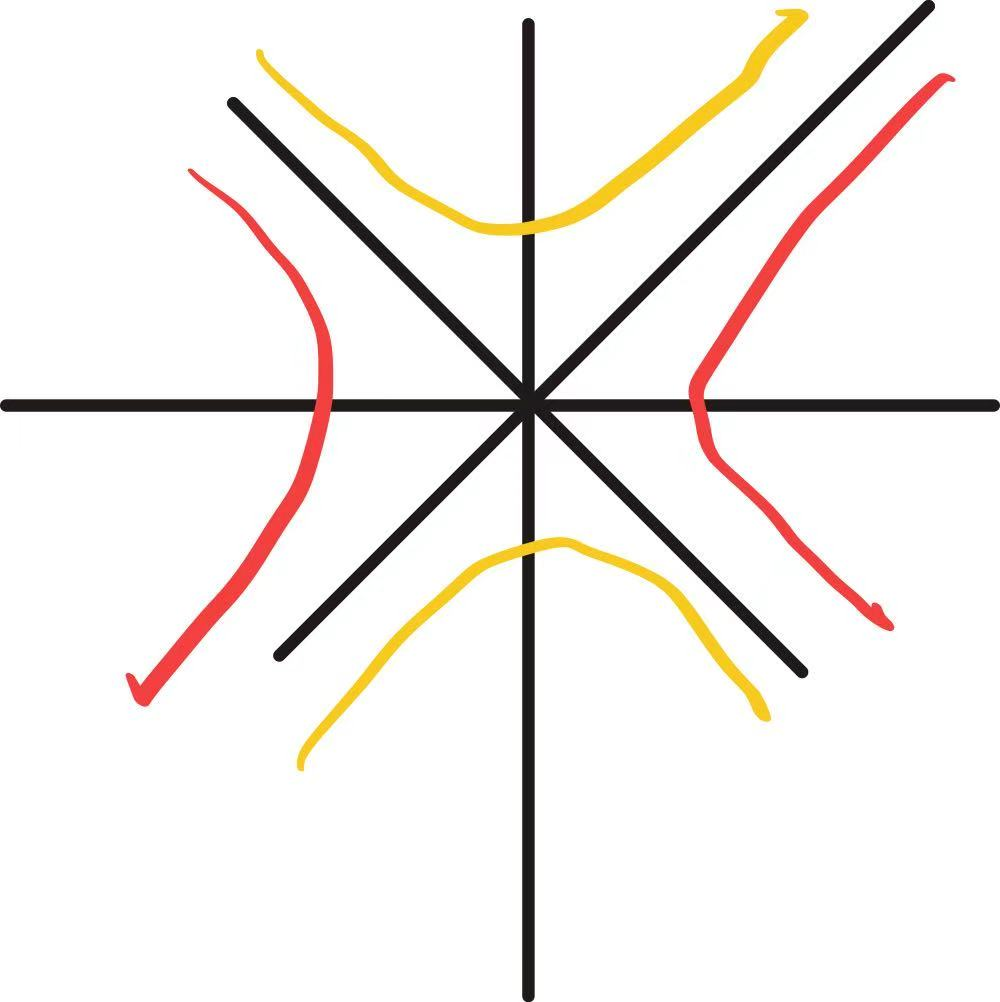
\includegraphics[height=3cm]{chapters/09/01/0201}}
                  \item $w=f(x,y,z)=x^2+y^2-z^2$\raisebox{-0.5\height}{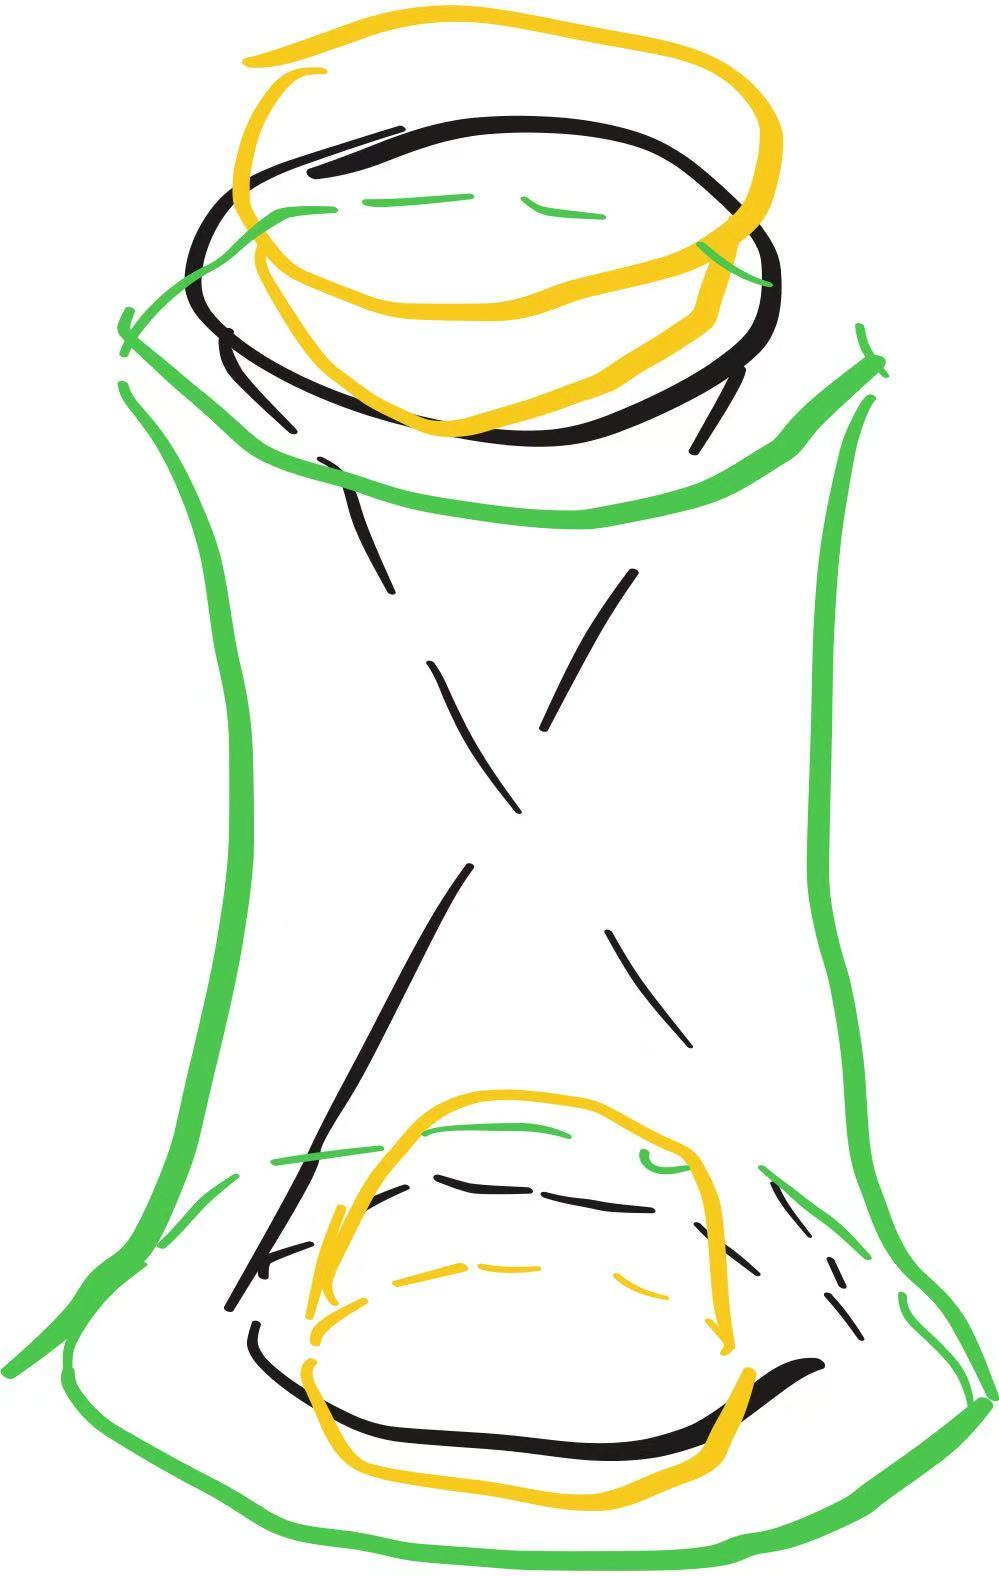
\includegraphics[height=3cm]{chapters/09/01/0202}}
              \end{itemize}
          \end{example}
\end{enumerate}

\paragraph{Vector-valued Functions}
\begin{align*}
    f:\,D\left(\subseteq\mathbb{R}^n\right) & \to\mathbb{R}^m                                                                                                  \\
    \left(x_1,\dots,x_n\right)              & \mapsto\left(y_1,\dots,y_n\right)=\left(f_1\left(x_1,\dots,x_n\right),\dots,f_n\left(x_1,\dots,x_n\right)\right)
\end{align*}

\begin{example}
    \begin{enumerate}
        \item $n=1,\,m=3$ parameterized curve
              \begin{align*}
                  \overrightarrow{r}:\,D\left(\subseteq\mathbb{R}\right) & \to\mathbb{R}^3                    \\
                  t                                                      & \mapsto\left(x(t),y(t),z(t)\right)
              \end{align*}
        \item $n=2,\,m=3$ parameterized surface in $\mathbb{R}^3$
              \begin{align*}
                  \overrightarrow{r}:\,D\left(\subseteq\mathbb{R}^2\right) & \to\mathbb{R}^3                          \\
                  \left(u,v\right)                                         & \mapsto\left(x(u,v),y(u,v),z(u,v)\right)
              \end{align*}
              \begin{example}
                  \begin{align*}
                      \overrightarrow{r}:\,[0,\pi]\times[0,2\pi] & \to\mathbb{R}^3                                                            \\
                      (\theta,\varphi)                           & \mapsto\left(\sin\theta\cos\varphi,\sin\theta\sin\varphi,\cos\theta\right)
                  \end{align*}is the spherical coordinate parameterization of the $S^2=\partial B(0,1)$
              \end{example}
        \item $n=m$ a one-to-one vector-valued function $f:\,D\left(\subseteq\mathbb{R}^b\right)\to\tilde{D}\left(\subseteq\mathbb{R}^b\right)$ is called a \emph{coordinate}.
    \end{enumerate}
\end{example}

\paragraph{\emph{Transformation}}

\begin{example}
    \begin{align*}
        \overrightarrow{r}:\,\mathbb{R}^2 & \to\mathbb{R}^2                                                                & x+iy=z              \\
        (x,y)                             & \mapsto\left(x^2-y^2,2xy\right)                                                & w=u+iv=z^2          \\
        (r,\theta)                        & \qquad=\left(r^2\cos 2\theta,r^2\sin 2\theta\right)\to\left(r^2,2\theta\right) & \text{Conformal 共形}
    \end{align*}

    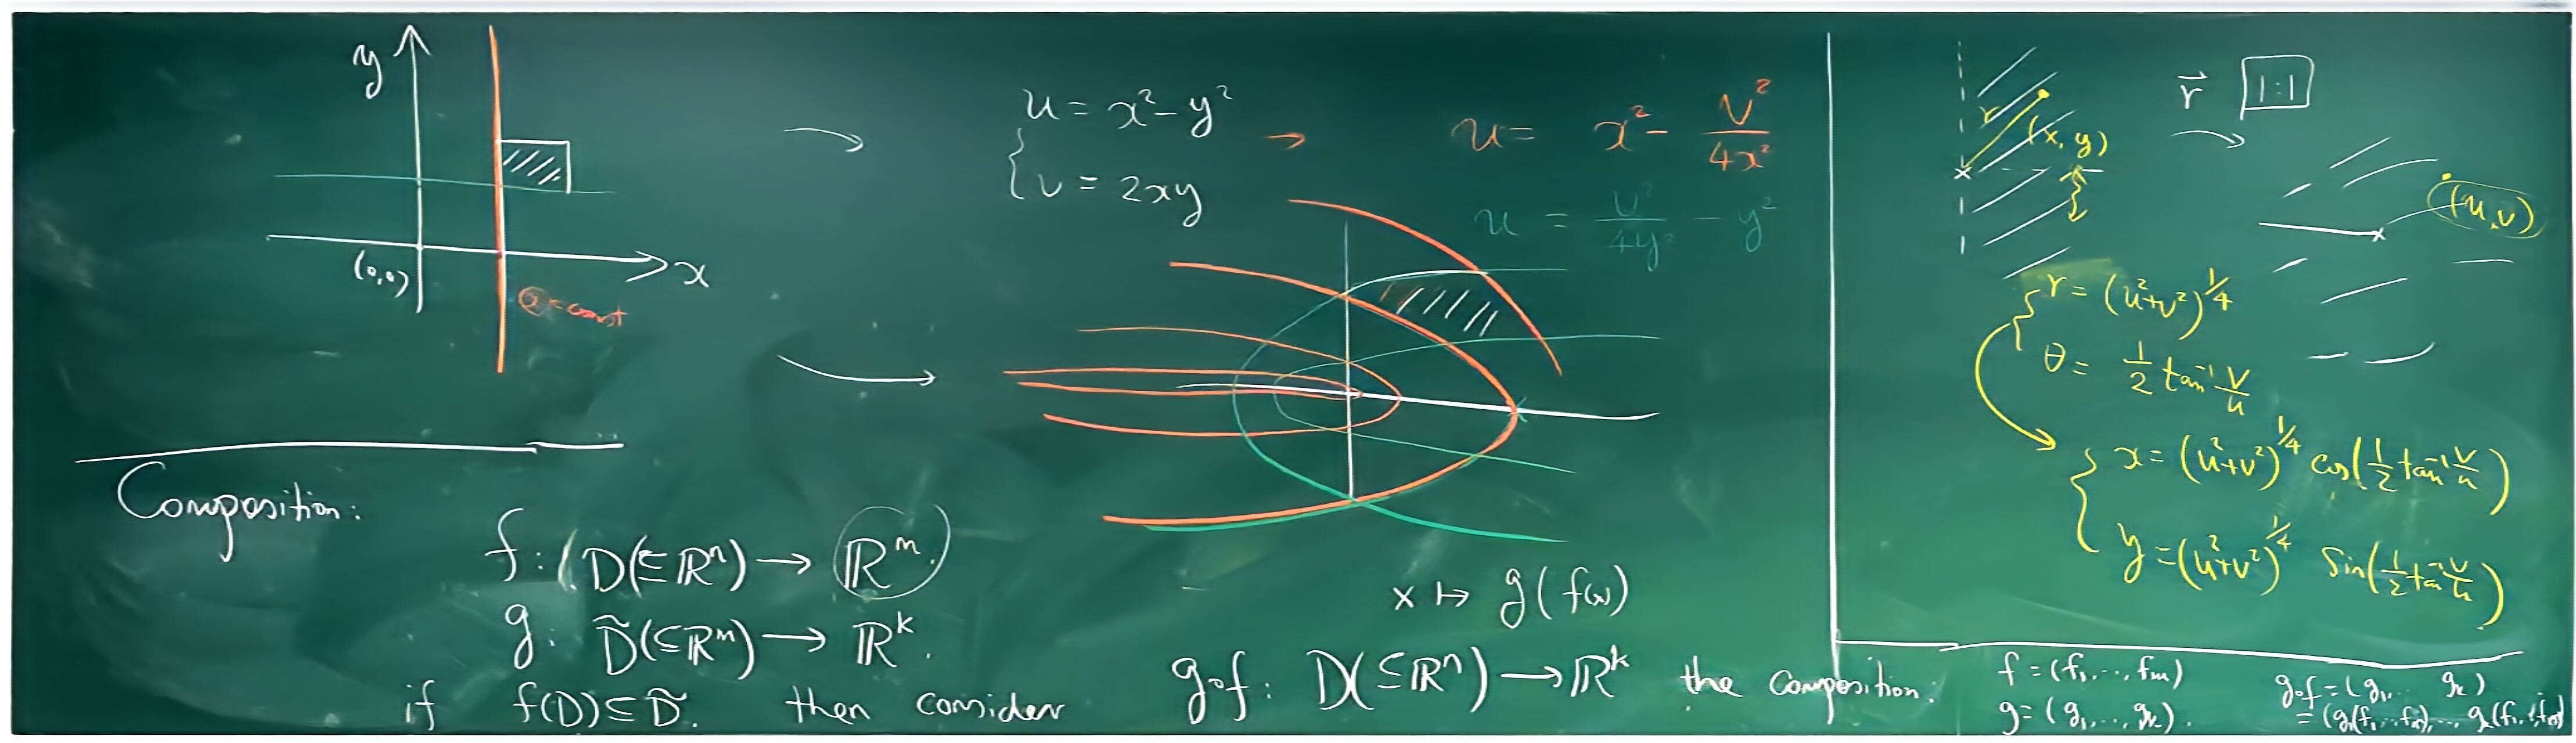
\includegraphics[width=0.9\linewidth]{chapters/09/01/0203}
\end{example}